\documentclass{beamer}

% theme definition
\usetheme{KU}

%\usepackage{natbib}
\usepackage{alltt}
%\usepackage{trust}
\usepackage{fixltx2e}
\usepackage{amsmath}
\usepackage{trust-spi}
\usepackage{tikz}
\usetikzlibrary{arrows,shadows, matrix}
\usepackage[underline=false]{pgf-umlsd}

\setbeamertemplate{blocks}[rounded][shadow=true]

\setbeamercolor{title}{fg=kublue}
\setbeamercolor{subtitle}{fg=kugray} 
\setbeamercolor{institute}{fg=kugray}
\setbeamercolor{frametitle}{fg=kublue}
\setbeamercolor{frametitle}{bg=white}
\setbeamercolor{framesubtitle}{fg=kugray}
\setbeamercolor{framesubtitle}{bg=white}
\setbeamercolor{item}{fg=black}
\setbeamercolor{subitem}{fg=kugray}
\setbeamercolor{itemize/enumerate subbody}{fg=kugray}
\setbeamercolor{block title}{bg=kublue}
\setbeamercolor{block title}{fg=white}
\setbeamercolor{block body}{bg=sand}
\setbeamercolor{block body}{fg=black}

\setbeamertemplate{footline}[frame number]

\usefonttheme{serif}

\newenvironment{fnverbatim}{\begin{alltt}\scriptsize}{\normalsize\end{alltt}}
\newcommand{\mean}[1]{\langle#1\rangle}
\newcommand{\rtime}{\ensuremath{\mathbb{R}^{0\leq}}}


%constants
\def \app {App}
\def \att {Att}
\def \ca {CA}
\def \mea {Meas}
\def \tp {TPM}
\def \pmask {PCR\textsubscript{m}}
\def \pcomp {PCR\textsubscript{c}}
\def \evd {d}
\def \eve {e}
\def \cacert {\sign {\public{AIK}}{CA}}
\def \exdata {\hash{(\eve, \nonce{\app}, \cacert ) }}
\def \aikh {AIK_h}

\def \req {R}
\def \resp {P}
\def \k {K}

\bibliographystyle{abbrv}

\logo{}

\title{ArmoredSoftware: Trust in the cloud}
\subtitle{Annual Demonstration}

\author{Dr. Perry Alexander, Dr. Andrew Gill, Dr. Prasad Kulkarni,
  Adam Petz, Paul Kline, Justin Dawson, Jason Gevargizian, Leon Searl,
  Edward Komp}

\date{{\color{kugray}January 15, 2015}}

% turns off navigation symbols
\setbeamertemplate{navigation symbols}{}

\institute{
    Information and Telecommunication Technology Center \\
    Electrical Engineering and Computer Science \\
    The University of Kansas \\
    \texttt{palexand@ku.edu,andygill@ku.edu,prasadk@ku.edu}}

\begin{document}

\begin{frame}
  \titlepage
\end{frame}

\logo{\pgfuseimage{jhwk4C_RF}}

\begin{frame}
  \frametitle{Outline}
  \tableofcontents
\end{frame}

\section{Introduction and Project Goals}
\subsection{Big Picture}

\begin{frame}
  \frametitle{Program Goals}
  \framesubtitle{Virtual Blinking Lights}
  \begin{block}{Trust in the Cloud}
    Provide new capabilities that establish and maintain trustworthy
    cloud-based application deployment
  \end{block}

  \begin{itemize}
  \item Establish trust among cloud components
    \begin{itemize}
    \item trust among cohorts of processes
    \item trust among processes and environment
    \end{itemize}
  \item Promote informed decision making
    \begin{itemize}
    \item data confidentiality can be confirmed
    \item execution and data integrity can be confirmed
    \end{itemize}
  \item Autonomous run-time response and reconfiguration
    \begin{itemize}
    \item responds to attack, failure, reconfiguration, and repair 
    \item response varies based on measurement
    \end{itemize}
  \end{itemize}
\end{frame}

\subsection{Implementation}

\begin{frame}
  \frametitle{Delivery Platform}
  \framesubtitle{Open source, standards compliant}

  \begin{itemize}
  \item Lightweight integration with existing cloud infrastructure
    \begin{itemize}
    \item OpenStack cloud infrastructure
    \item Xen+XSM VM infrastructure
    \item Fedora, HotSpot JVM, GHC
    \end{itemize}
  \item Trusted Computing Group standards compliant
    \begin{itemize}
    \item Trusted Platform Module 1.2
    \item TCG vTPM (in principle)
    \item Trusted OS infrastructure
    \end{itemize}
  \item Standard communication mechanisms
    \begin{itemize}
    \item JSON structures for all exchanged data
    \item \textsl{vchan} for on-platform communication
    \item TCP/IP for off-platform communication
    \end{itemize}
  \end{itemize}
\end{frame}

\begin{frame}
  \frametitle{New Technologies}
  \begin{itemize}
  \item Trustworthy protocol execution
    \begin{itemize}
    \item executable protocol representation
    \item protocol execution generates evidence of trustworthiness
    \item highly focused protocols
    \item strand space formal semantics
    \end{itemize}
  \item Application specific measurement
    \begin{itemize}
    \item managed and traditional execution environments
    \item compile-time assistance for measurer synthesis
    \item specialized measurement bundled with applications
    \end{itemize}
  \item Attestation driven cloud application and data management
    \begin{itemize}
    \item health monitoring
    \item problem mitigation
    \item application migration
    \item access control
    \end{itemize}
  \end{itemize}
\end{frame}

\begin{frame}
  \frametitle{Research \& Development Plan}
  \begin{itemize}
  \item Development and integrate measurement capabilities
    \begin{itemize}
    \item hosted languages (Java)
    \item traditional compiled languages (C, C++)
    \item integrate with environment measurers (Xen,OpenStack,OS)
    \end{itemize}
  \item Develop attestation capabilities
    \begin{itemize}
    \item flexible, user configurable protocol representation
    \item measured protocol execution
    \item protocol execution appraisal
    \end{itemize}
  \item Develop infrastructure trust argument
    \begin{itemize}
    \item develop lightweight vTPM infrastructure supporting mobility
    \item launch from known roots of trust
    \item maintain trust evidence at run time
    \item maintain trust over migration
    \end{itemize}
  \end{itemize}
\end{frame}

\begin{frame}
  \frametitle{Research \& Development Plan}
  \begin{itemize}
  \item Automated synthesis and verification
    \begin{itemize}
    \item measurer synthesis at application compile time
    \item automated evidence appraisal from protocols
    \item formal trust argument
    \end{itemize}
  \item Demonstrations
    \begin{itemize}
    \item initial simple infrastructure demonstrations
    \item cloud-based ``big data'' environment demonstration
    \item federated trust demonstration
    \item \emph{demonstrations as discovered/directed}
    \end{itemize}
  \item Scale up and roll out
    \begin{itemize}
    \item integration with Xen, OpenStack, Linux
    \item installation management and packaging
    \item effective web presence
    \end{itemize}
  \end{itemize}
\end{frame}

\begin{frame}
  \frametitle{Armored Application Architecture}
  \begin{columns}[c]
    \column{.60\textwidth}
    \begin{itemize}
    \item Focus is user-space applications
    \item Assesses the cloud infrastructure and environment
    \item Attests to the state of its application
    \item High-assurance, lightweight infrastructure
    \item Influenced by the \emph{Trusted Research Platform} and
      \emph{Principles of Remote Attestation}
    \end{itemize}
    \column{.40\textwidth}
    \begin{center}
    \includegraphics[width=0.55\textwidth]{figures/architecture.pdf}
    \end{center}
  \end{columns}
\end{frame}

\begin{frame}
  \frametitle{System-Level Architecture}
  \begin{center}
  \includegraphics[width=0.9\textwidth]{figures/system.pdf}
  \end{center}
\end{frame}

\section{Prototype demonstration and discussion}

\begin{frame}
  \frametitle{What We Are Demonstrating}
  
  \begin{itemize}
  \item Execution of a CA-based Attestation Protocol
    \begin{itemize}
    \item Attestation request
    \item Protocol execution
    \item Evidence appraisal
    \end{itemize}
  \item Major architectural subsystems
    \begin{itemize}
    \item Appraiser
    \item Attestation Manager
    \item Measurer
    \item Instrumented JVM
    \item vTPM and Certificate Authority
    \end{itemize}
  \item Anomaly Detection
    \begin{itemize}
    \item Bad signatures and PCRs
    \item Bad CA certificates
    \item Bad quotes and AIKs
    \item Bad measurements
    \end{itemize}
  \end{itemize}
\end{frame}

\begin{frame}[fragile]
  \frametitle{Abstract CA-Based Attestation Protocol}

  \begin{center}

    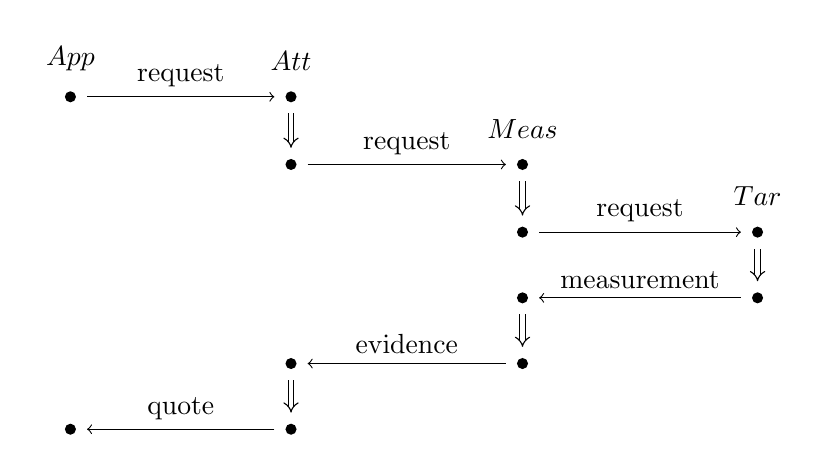
\begin{tikzpicture}[
    implies/.style={double,double equal sign distance,-implies},
    dot/.style={shape=circle,fill=black,minimum size=4pt,
      inner sep=0pt,outer sep=4pt}]

    \matrix[matrix of nodes] {
      |[dot,label=above:$\app$] (A1)| {}
      &[2.0cm] |[dot,label=above:$\att$] (B1)| {}
      &[2.0cm] |[] (M1)| {} 
      &[2.0cm] |[] (T1)| {}\\[0.05cm]
      |[] (A2)| {}
      &|[dot] (B2)| {}
      &|[dot,label=above:$\mea$] (M2)| {} 
      &|[] (T2)| {}\\[0.05cm]
      |[] (A3)| {}
      &|[] (B3)| {}
      &|[dot] (M3)| {} 
      &|[dot,label=above:$Tar$] (T3)| {}\\[0.6cm]
      |[] (A4)| {}
      &|[] (B4)| {}
      &|[dot] (M4)| {} 
      &|[dot] (T4)| {}\\[0.6cm]
      |[] (A5)| {}
      &|[dot] (B5)| {}
      &|[dot] (M5)| {} 
      &|[] (T5)| {}\\[0.6cm]
      |[dot] (A6)| {}
      &[2.0cm] |[dot] (B6)| {}
      &[2.0cm] |[] (M6)| {} 
      &[2.0cm] |[] (T6)| {}\\
    };
    \draw (A1) edge[->] node[above] {request} (B1);
    \draw (B2) edge[->] node[above] {request} (M2)
           edge[implies,implies-] (B1);
    \draw (M3) edge[->] node[above] {request} (T3)
           edge[implies,implies-] (M2);
    \draw (T4) edge[->] node[above] {measurement} (M4)
           edge[implies,implies-] (T3);
    \draw (M5) edge[->] node[above] {evidence} (B5)
           edge[implies,implies-] (M4);
    \draw (B6) edge[->] node[above] {quote} (A6)
           edge[implies,implies-] (B5);
    \end{tikzpicture}

    \end{center}

\end{frame}

\begin{frame}
  \frametitle{Abstract CA-Based Attestation Protocol}
  
  \begin{footnotesize}
  \begin{sequencediagram}
    \newthread[white]{appr}{Appraiser}
    \newinst[1.0]{attest}{Attestation}
    \newinst[1.5]{meas}{Measurer}
    \newinst[1.0]{app}{Application}
    
    \begin{call}{appr}{Request}{attest}{Evidence}
      \begin{callself}{attest}{Protocol Selection}{}
      \end{callself}
      \begin{call}{attest}{Request}{meas}{Value}
        \begin{call}{meas}{Measurement}{app}{Value}
        \end{call}
      \end{call}
      \begin{callself}{attest}{Quote Assembly}{}
      \end{callself}
    \end{call}
    \begin{callself}{appr}{Appraisal}{Execute Decision}
    \end{callself}
  \end{sequencediagram}
  \end{footnotesize}

\end{frame}

\begin{frame}
  \frametitle{Message List Representation}
  \begin{small}
  \begin{align*}
  & \sndmsg {\app}{\att} {\evd, \nonce{\app}, \pmask} {\channel {\app \att}}  & \\
  & \sndmsg{\att}{\tp} {make\_and\_load\_identity} {\channel {\att \tp}} & \\
  & \sndmsg{\tp}{\att} {\public{AIK}, \aikh} {\channel {\tp \att}} & \\
  & \sndmsg{\att}{\ca} {\att, \public{AIK}} {\channel {\att \ca}} & \\
  & \sndmsg{\ca}{\att} {\encrypt{K, \hash{AIK}}{EK}, \encrypt{\cacert}{K}} {\channel {\ca \att}}& \\
  & \sndmsg{\att}{\tp} {activate\_identity({\aikh, \hash{AIK})}} {\channel {\att \tp}} & \\
  & \sndmsg{\tp}{\att} {K} {\channel {\tp \att}} & \\
  & \sndmsg{\att}{\mea} {\evd} {\channel {\att \mea}} & \\
  & \sndmsg{\mea}{\att} {\eve} {\channel {\mea \att}} & \\
  & \sndmsg{\att}{\tp} {quote(\;{AIK\textsubscript{h}, \pmask, \exdata}\;)} {\channel {\att \tp}} & \\
  & \sndmsg{\tp}{\att} {\pcomp, \sign{\hash{\pcomp}, \exdata}{AIK}} {\channel {\tp \att}} & \\
  & \sndmsg{\att}{\app} {\eve, \nonce{\app}, \pcomp, \cacert} {\channel {\att \app}} & \\
  & \sndmsg{\att}{\app} {\sign{\hash{\pcomp}, \exdata}{AIK}} {\channel {\att \app}} & 
\end{align*}
\end{small}
\end{frame}

\subsection{Refine big picture to current demo}

\begin{frame}[fragile]
  \frametitle{Strand Space Diagram Representation}

  \begin{tiny}
  \begin{tikzpicture}[
    implies/.style={double,double equal sign distance,-implies},
    dot/.style={shape=circle,fill=black,minimum size=4pt,
      inner sep=0pt,outer sep=4pt}]

    \matrix[matrix of nodes] {
      |[dot,label=above:$\app$] (A1)| {}
      &[4.0cm] |[dot,label=above:$\att$] (B1)| {}
      &[1.95cm] |[] (M1)| {} 
      &[1.95cm] |[] (T1)| {}
      &[0.5cm] |[] (C1)| {}\\[0.05cm]
      & |[dot] (B2)| {}
      &
      & |[dot,label=above:$\tp$] (T2)| {}\\[0.5cm]
      &
      |[dot] (B3)| {}
      &
      & |[dot] (T3)| {}\\  [0.05cm]
      &
      |[dot] (B4)| {}
      &
      &
      & |[dot,label=above:$\ca$] (C4)| {} \\ [0.5cm]
      &
      |[dot] (B5)| {}
      &
      &
      & |[dot] (C5)| {} \\ [0.5cm]
      &
      |[dot] (B6)| {}
      &
      & |[dot] (T6)| {} \\ [0.5cm]
      &
      |[dot] (B7)| {}
      &
      & |[dot] (T7)| {} \\ [0.05cm]
      &
      |[dot] (B8)| {}
      & |[dot,label=above:$\mea$] (M8)| {} \\ [0.5cm]
      &
      |[dot] (B9)| {}
      & |[dot] (M9)| {} \\ [0.5cm]
      &
      |[dot] (B10)| {}
      &
      & |[dot] (T10)| {} \\ [0.5cm]
      &
      |[dot] (B11)| {}
      &
      & |[dot] (T11)| {} \\ [0.5cm]
      |[dot] (A12)| {}
      & |[dot] (B12)| {} \\ [0.5cm]
      |[dot] (A13)| {}
      & |[dot] (B13)| {} \\ [0.5cm]
};
\draw (A1) edge[->] node[above] {$\evd, \nonce{\app}, \pmask$} (B1);
\draw (B2) edge[->] node[above] {$make\_and\_load\_identity$} (T2)
           edge[implies,implies-] (B1);
\draw (T3) edge[->] node[above] {$\aikh$} (B3)
           edge[implies,implies-] (T2);
\draw (B4) edge[->] node[above] {$\public{AIK}$} (C4)
           edge[implies,implies-] (B3);
\draw (C5) edge[->] node[above] {$\encrypt{K, \hash{\public{AIK}}}{EK}, \crypt{\cacert}{K}$} (B5)
           edge[implies,implies-] (C4);
\draw (B6) edge[->] node[above] {$activate\_identity(\aikh, \encrypt{K, \hash{\public{AIK}}}{EK})$} (T6)
           edge[implies,implies-] (B5);
\draw (T7) edge[->] node[above] {$K$} (B7)
           edge[implies,implies-] (T6);
\draw (B8) edge[->] node[above] {$\evd$} (M8)
           edge[implies,implies-] (B7);
\draw (M9) edge[->] node[above] {$\eve$} (B9)
           edge[implies,implies-] (M8);
\draw (B10) edge[->] node[above] {$quote(\;\aikh, \pmask, \exdata \;)$} (T10)
% quote(\;{AIK\textsubscript{h}, \pmask, \exdata}\;)
           edge[implies,implies-] (B9);
\draw (T11) edge[->] node[above] {$\pcomp, \sign{\hash{\pcomp}, \exdata}{AIK}$} (B11)
% \pcomp, sig(\hash{\pcomp}, ed) AIK
           edge[implies,implies-] (T10);
\draw (B12) edge[->] node[above] {$\eve, \nonce{\app}, \pcomp, \cacert$} (A12)
% \eve, \nonce{\app}, \pcomp, \cacert
           edge[implies,implies-] (B11);
\draw (B13) edge[->] node[above] {$\sign{\hash{\pcomp}, \exdata}{AIK}$} (A13) 
% sig(hash(\pcomp), ed) AIK
           edge[implies,implies-] (B12);
\end{tikzpicture}
\end{tiny}
\end{frame}

\subsection{Protocol Execution}

\begin{frame}[fragile]
  \frametitle{Attestation Request}
  \begin{center}
    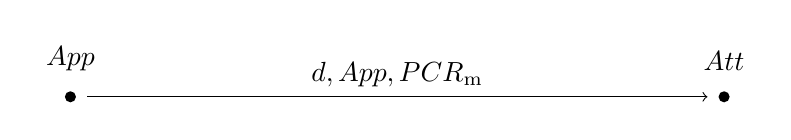
\begin{tikzpicture}[
      implies/.style={double,double equal sign distance,-implies},
      dot/.style={shape=circle,fill=black,minimum size=4pt,
        inner sep=0pt,outer sep=4pt}]
      \matrix[matrix of nodes] {
        |[dot,label=above:$\app$] (A1)| {}
        &[7.5cm] |[dot,label=above:$\att$] (B1)| {} \\ [1.0cm]
      };
      \draw (A1) edge[->] node[above] {$\evd, \nonce{\app}, \pmask$} (B1);
    \end{tikzpicture}
  \end{center}

    \begin{itemize}
    \item Initiate with an attestation request
      \begin{itemize}
      \item $d$ abstractly defines desired evidence
      \item $\nonce{\app}$ is the appraiser's nonce
      \item $\pmask$ selects PCRs
      \end{itemize}
    \item Attestation agent selects and executes protocol based on request
    \end{itemize}
\end{frame}

\begin{frame}[fragile]
  \frametitle{Generating and Certifying an AIK}

  \begin{columns}[c]
    \column{.45\textwidth}
    \begin{small}
    \begin{itemize}
    \item Request a new $AIK$ from TPM (optional)
    \item Receive $AIK$ handle
    \item Request $\public{AIK}$ signed by CA ($AIK$ cert)
    \item Receive $AIK$ cert encrypted with session key $K$
    \item Receive $K$ encrypted with public $EK$
    \end{itemize}
    \end{small}
    \column{.55\textwidth}
    \begin{small}
    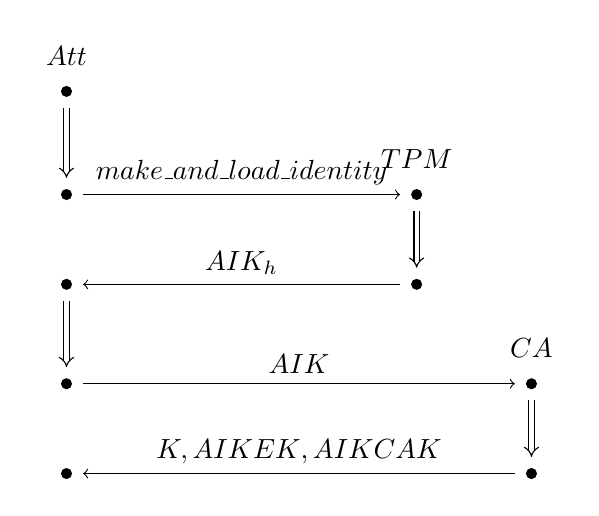
\begin{tikzpicture}[
      implies/.style={double,double equal sign distance,-implies},
      dot/.style={shape=circle,fill=black,minimum size=4pt,
        inner sep=0pt,outer sep=4pt}]
      \matrix[matrix of nodes] {
        |[dot,label=above:$\att$] (B1)| {}
        &[3.5cm] |[] (T1)| {}
        &[0.5cm] |[] (C1)| {}\\[0.5cm]
        |[dot] (B2)| {}
        &|[dot,label=above:$\tp$] (T2)| {}\\[1.0cm]
        |[dot] (B3)| {}
        & |[dot] (T3)| {}\\  [0.5cm]
        |[dot] (B4)| {}
        &
        & |[dot,label=above:$\ca$] (C4)| {} \\ [1.0cm]
        |[dot] (B5)| {}
        &
        & |[dot] (C5)| {} \\ [0.5cm]
      };
\draw (B2) edge[->] node[above] {$make\_and\_load\_identity$} (T2)
           edge[implies,implies-] (B1);
\draw (T3) edge[->] node[above] {$\aikh$} (B3)
           edge[implies,implies-] (T2);
\draw (B4) edge[->] node[above] {$\public{AIK}$} (C4)
           edge[implies,implies-] (B3);
\draw (C5) edge[->] node[above] {$\encrypt{K, \hash{\public{AIK}}}{EK}, \crypt{\cacert}{K}$} (B5)
           edge[implies,implies-] (C4);
    \end{tikzpicture}
    \end{small}
  \end{columns}
\end{frame}

\begin{frame}[fragile]
  \frametitle{Activating the AIK}

  \begin{center}
    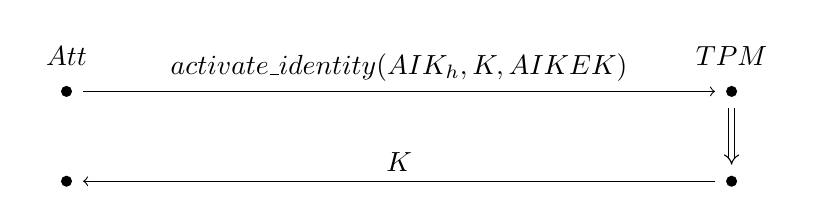
\begin{tikzpicture}[
      implies/.style={double,double equal sign distance,-implies},
      dot/.style={shape=circle,fill=black,minimum size=4pt,
        inner sep=0pt,outer sep=4pt}]
      \matrix[matrix of nodes] {
        |[dot,label=above:$\att$] (B6)| {}
        &[7.5cm] |[dot,label=above:$\tp$] (T6)| {} \\ [1.0cm]
        |[dot] (B7)| {}
        &|[dot] (T7)| {} \\
      };
\draw (B6) edge[->] node[above] {$activate\_identity(\aikh, \encrypt{K, \hash{\public{AIK}}}{EK})$} (T6);
\draw (T7) edge[->] node[above] {$K$} (B7)
           edge[implies,implies-] (T6);
    \end{tikzpicture}
  \end{center}

    \begin{itemize}
    \item Request TPM decryption of the $AIK$ cert
    \item Receive $K$ used to decrypt signed public $AIK$
    \item Only TPM can gain access to $K$
    \item Only TPM can obtain signed, public $AIK$
    \item Oddly, No manipulation of the $AIK$ in this ``activation''
      process
    \end{itemize}

\end{frame}

\begin{frame}[fragile]
  \frametitle{Measurement}

  \begin{center}
    \begin{tikzpicture}[
      implies/.style={double,double equal sign distance,-implies},
      dot/.style={shape=circle,fill=black,minimum size=4pt,
        inner sep=0pt,outer sep=4pt}]
      \matrix[matrix of nodes] {
        |[dot,label=above:$\att$] (B8)| {}
        &[7.5cm] |[dot,label=above:$\mea$] (M8)| {} \\ [1.0cm]
        |[dot] (B9)| {}
        &|[dot] (M9)| {} \\
      };
      \draw (B8) edge[->] node[above] {$\evd$} (M8);
      \draw (M9) edge[->] node[above] {$\eve$} (B9)
      edge[implies,implies-] (M8);
    \end{tikzpicture}
  \end{center}

    \begin{itemize}
    \item Request information from measurer
    \item Receive evidence $e$ from measurer
    \item $d$ is abstract allowing protocol reuse
    \item Most protocols make many requests of the measurer
    \end{itemize}

\end{frame}

\begin{frame}[fragile]
  \frametitle{Generating a Quote}

  \begin{center}
    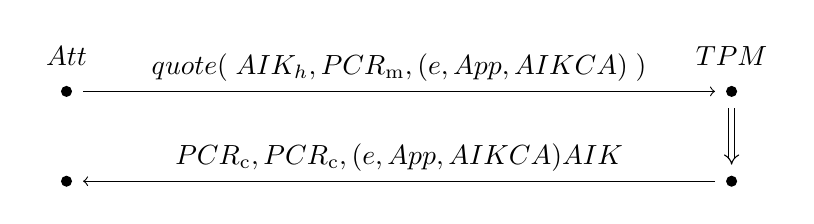
\begin{tikzpicture}[
      implies/.style={double,double equal sign distance,-implies},
      dot/.style={shape=circle,fill=black,minimum size=4pt,
        inner sep=0pt,outer sep=4pt}]
      \matrix[matrix of nodes] {
        |[dot,label=above:$\att$] (B10)| {}
        &[7.5cm] |[dot,label=above:$\tp$] (T10)| {} \\ [1.0cm]
        |[dot] (B11)| {}
        &|[dot] (T11)| {} \\
      };
\draw (B10) edge[->] node[above] {$quote(\;\aikh, \pmask, \exdata \;)$} (T10);
% quote(\;{AIK\textsubscript{h}, \pmask, \exdata}\;)
\draw (T11) edge[->] node[above] {$\pcomp, \sign{\hash{\pcomp}, \exdata}{AIK}$} (B11)
% \pcomp, sig(\hash{\pcomp}, ed) AIK
           edge[implies,implies-] (T10);
    \end{tikzpicture}
  \end{center}

    \begin{itemize}
    \item Request a quote from the TPM
      \begin{itemize}
      \item $AIK$ identifies the signing $AIK$
      \item $PCR_m$ identifies desired PCRs
      \item $\exdata$ guarantees integrity of returned evidence
      \end{itemize}
    \item Receive quote from TPM
      \begin{itemize}
      \item $\pcomp$ is PCR composite built from requested PCRs
      \item $\sign{\hash{\pcomp}, \exdata}{AIK}$ is the signed quote
      \end{itemize}
    \end{itemize}

\end{frame}

\begin{frame}[fragile]
  \frametitle{Appraisal}

  \begin{center}
    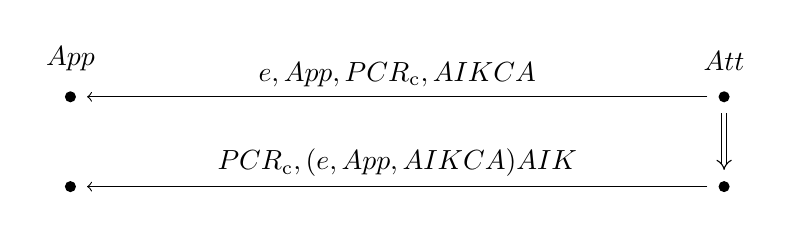
\begin{tikzpicture}[
      implies/.style={double,double equal sign distance,-implies},
      dot/.style={shape=circle,fill=black,minimum size=4pt,
        inner sep=0pt,outer sep=4pt}]
      \matrix[matrix of nodes] {
        |[dot,label=above:$\app$] (A12)| {}
        &[7.5cm] |[dot,label=above:$\att$] (B12)| {} \\ [1.0cm]
        |[dot] (A13)| {}
        &|[dot] (B13)| {} \\
      };
      \draw (B12) edge[->] node[above] {$\eve, \nonce{\app}, \pcomp, \cacert$} (A12);
      % \eve, \nonce{\app}, \pcomp, \cacert
\draw (B13) edge[->] node[above] {$\sign{\hash{\pcomp}, \exdata}{AIK}$} (A13) 
% sig(hash(\pcomp), ed) AIK
           edge[implies,implies-] (B12);

    \end{tikzpicture}
  \end{center}

    \begin{itemize}
    \item Receive evidence from the attestation manager
      \begin{itemize}
      \item evidence
      \item original nonce
      \item PCR composite 
      \item signed $\public{AIK}$
      \end{itemize}
    \item Receive TPM quote from the attestation manager
      \begin{itemize}
      \item hash of all evidence
      \item PCR composite
      \item signed by $\private{AIK}$
      \end{itemize}
    \item Evaluate evidence and quote
    \end{itemize}

\end{frame}

\subsection{Appraisal}

\begin{frame}
  \frametitle{Evidence Appraisal}

  \begin{center}
    {\color{kublue}Demonstration detects failure of all aspects of attestation}
  \end{center}

  \[\eve, \nonce{\app}, \pcomp, \cacert\]

  \begin{itemize}
  \item $\eve$ -- evidence gathered from running application
  \item $\nonce{\app}$ -- prevents replay
  \item $\pcomp$ -- evidence in the form or PCR data from the vTPM
  \item $\cacert$ -- ensures validity of $\public{AIK}$
  \end{itemize}

  \[\sign{\hash{\pcomp}, \exdata}{AIK}\]

  \begin{itemize}
  \item $\pcomp$ -- hash ensures integrity of PCR data
  \item $\exdata$ -- hash ensures integrity of evidence, nonce, and
    signed $\public{AIK}$
  \end{itemize}

\end{frame}

\subsection{Attestation Protocol Execution}

\begin{frame}
  \frametitle{Attestation Protocol Execution}
\end{frame}

\subsection{Measurement}

\begin{frame}
  \frametitle{3-4 Slides on Measurement}
\end{frame}

\subsection{Communication}

\begin{frame}
  \frametitle{2-3 Slides on Communication Mechanisms}
\end{frame}
\begin{frame}{CA communication}
Shared notion of AIKCertRequest, AIKCert, and CAResponse JSON structures.
$\linebreak$
$\linebreak$
Attester
\begin{itemize}
\item {creates an AIKCertRequest (containing attester $ID$, \public{AIK}) and converts to JSON}
\item {JSON sent as POST request to \ca{} running as web server}
\end{itemize}
$\linebreak$
Certificate Authority
\begin{itemize}
\item {POST body bytes $\rightarrow$ UTF8 $\rightarrow$ JSON $\rightarrow$ AIKCertRequest}
\item {looks up \public{EK} associated with $ID$ in sql database}
\item {AIKCert $=$ \public{AIK} signed with \private{CA} }
\item {generates key $K$ and encrypts with \public{EK}}
\item {AIKCert encrypted with $K$}
\item {both wrapped in a CAResponse, converted to JSON and sent as response. }

\end{itemize}

\end{frame}

\begin{frame}{\ca{} communication continued}
Properties
\begin{itemize}
\item {\ca{} only responds to receiving an $AIKCertRequest_{JSON}$ }
\item {The CACert can \emph{only} be decrypted by knowing $K$ (and therefore \private{EK})}
\end{itemize}
$\linebreak$
Appraiser Knowledge after receiving Cert:
\begin{itemize}
\item {signature on $AIK$ ensures it was \ca{} who generated signature
}
+
\item {only an entity knowing \private{EK} could decrypt and send the CACert
}
$\linebreak$
=
\item {\textbf{Attester is using a registered TPM}}

\end{itemize}

\end{frame}


\begin{frame}
  \frametitle{Current Status}

  \begin{center}
  \emph{\color{kublue}Completed four demonstrations culminating in
    running an attestation protocol in response to an attestation
    request.}
  \end{center}

  \begin{itemize}
  \item Attestation and Appraisal development
    \begin{itemize}
    \item CA-Based attestation protocol execution example
    \item integration with Berlios TPM 1.2 emulator
    \item simple dynamic appraisal of attestation results
    \end{itemize}
  \item Measurement development
    \begin{itemize}
    \item on demand Java program measurement
    \item HotSpot-based Java VM run time measurements
    \item standard mechanism for extending measurement capabilities
    \end{itemize}
  \item Communication infrastructure
    \begin{itemize}
    \item vchan, TCP/IP and socket communication infrastructure
    \item language-based interface with TPM 1.2
    \item JSON-based data exchange formats
    \item initial certificate authority API
    \end{itemize}
  \end{itemize}
\end{frame}

\section{Short term goals and milestones}

\begin{frame}
  \frametitle{Goals and Milestones for 2015}

  \begin{itemize}
  \item Push to the cloud
  \item Establish roots of trust and trust argument
  \item Executable protocol representation and protocol semantics
  \item Operational, integrated vTPM prototype
  \item Name Server / Certificate Authority prototype
  \item More capable measurement
  \item Downloadable demonstration
  \end{itemize}
\end{frame}

\section{Questions and guidance}

\begin{frame}
  \frametitle{Questions and Guidance}

  \begin{itemize}
  \item What problems are interesting?
  \item What problem would be a nice attention grabber?
  \item What should we be watching and integrating with?
  \end{itemize}
\end{frame}

\nocite{Coker::Principles-of-R,Haldar:04:Semantic-Remote,Fabrega:1999aa}

\begin{frame}
  \frametitle{References}
  \bibliography{demo14}
\end{frame}

\end{document}

